% IEEE conference paper — leakage-controlled nested-LOSO comparison of
% spiking / recurrent / attention autoencoders on FSDD.
% Revision of rejected submission 71 (Guayaquil); retargeted to the next congress.
\documentclass[conference]{IEEEtran}
\usepackage{amsmath,amsfonts,amssymb}
\usepackage{microtype}
\usepackage{graphicx}
\usepackage{tikz}
\usetikzlibrary{shapes.geometric,arrows.meta,positioning}
\usepackage{pgfplots}
\pgfplotsset{compat=1.18}
\usepackage{pgfplotstable}
\usepackage{cite}
\usepackage{balance}
\usepackage{booktabs}
\usepackage[english]{babel}

\title{Spiking, Recurrent, and Attention Autoencoders for
Temporal Signals: A Leakage-Controlled Nested Cross-Validation Comparison}

\author{André Furlan\\Instituto de Biociências, Letras e Ciências Exatas - UNESP\\ andre.furlan@unesp.br}

\begin{document}
\maketitle
\sloppy
\emergencystretch=3em

\begin{abstract}

\par Spiking Neural Networks (SNNs) promise low-power temporal signal
processing through event-driven, sparse computation, but their use as
autoencoders for waveform reconstruction lacks a controlled, leakage-free
empirical comparison against modern non-spiking baselines. We compare four
trained autoencoder families --- a spiking autoencoder (SNN-AE), an LSTM
autoencoder (LSTM-AE), a GRU autoencoder (GRU-AE), and a bottlenecked
Transformer autoencoder (Transformer-AE) without encoder--decoder
cross-attention --- under three spike-encoding front ends (direct, Poisson,
latency), together with PCA and mean-frame linear reference points. All models
share a single C++/CPU harness \cite{furlan2026doi} for matched timing and a
transparent operation-count cost budget. Evaluation uses \emph{nested six-fold
leave-one-speaker-out cross-validation} on the Free Spoken Digit Dataset (FSDD)
\cite{jackson2018fsdd}: no source recording or speaker crosses a split, and SNN
hyperparameters are selected inside each fold on the held-out validation speaker
only, then retrained on the combined training and validation data before a
single evaluation on the untouched test speaker. Model differences are assessed
with a recording-level paired analysis (bootstrap confidence intervals over
recordings, Wilcoxon signed-rank, Holm--Bonferroni), with speaker-level
($n=6$) and seed-level results reported as generalization- and
optimization-robustness evidence. We report reconstruction quality
(MSE, MAE, $R^2$) as mean $\pm$ standard deviation over seeds, a raw
per-class operation count as the primary cost figure (with a weighted proxy
as a labelled sensitivity analysis), the self-attention $O(T^2 d_{\mathrm{model}})$
interaction cost, and real parameter counts. The harness and profiles are
released for reproduction.
\end{abstract}

\begin{IEEEkeywords}
spiking neural networks, LSTM, GRU, Transformer, autoencoder,
temporal signals, surrogate gradients, nested cross-validation,
data leakage, audio signal processing
\end{IEEEkeywords}

% ─────────────────────────────────────────────────────────────
\section{Introduction}

\par One-dimensional temporal signals such as audio waveforms, biosignals, and
sensor streams often need to be processed and interpreted in low-power
embedded systems where the energy budget is a primary constraint.

\par Autoencoders for such signals must learn compact latent representations
efficiently and accurately reconstruct the original sequence.

\par Long Short-Term Memory (LSTM) autoencoders are a well-established baseline
for sequence reconstruction \cite{sutskever2014sequence,hochreiter1997long},
but their dense matrix operations are computationally expensive.
Spiking Neural Networks (SNNs) otherwise communicate via sparse binary events and
perform synaptic updates only when spikes occur, offering potential energy
reduction on general-purpose and neuromorphic hardware
\cite{maass1997networks,pfeiffer2018deep,gerstner2002spiking}.

\par Training SNNs for reconstruction requires backpropagation through
non-differentiable spike functions which behave like step functions.
Surrogate gradient methods \cite{neftci2019surrogate,zenke2018superspike} enable
end-to-end gradient-based training and have produced competitive SNN
classification performance \cite{eshraghian2023training,pfeiffer2018deep}.
However, a controlled study of SNN autoencoders for temporal signal
reconstruction --- compared against several modern non-spiking baselines, under
an evaluation protocol that provably prevents information from the test signals
leaking into training or hyperparameter selection --- is lacking.

\par Evaluation rigor is the crux. When fixed-length windows from all recordings
are pooled, shuffled, and split, windows from the same utterance --- and the
same speaker --- appear in both training and validation, so reported errors
partly measure memorization of speaker- and recording-specific waveform detail.
Speaker identity is the natural unit of generalization for a spoken-digit
benchmark, and FSDD provides only six speakers, which also bounds how strong any
population-level claim can be.

\par This paper addresses these gaps with four contributions:
\begin{enumerate}
  \item A leakage-controlled protocol: \emph{nested six-fold
        leave-one-speaker-out cross-validation} on FSDD \cite{jackson2018fsdd}
        in which no source recording or speaker crosses a split and SNN
        hyperparameters are selected on the inner validation speaker only.
  \item A comparison of four trained autoencoder families under three input
        encodings --- SNN-AE, LSTM-AE, GRU-AE, and a bottlenecked
        Transformer-AE without encoder--decoder cross-attention --- plus PCA
        and mean-frame linear reference points, all on one matched C++/CPU
        harness \cite{furlan2026doi,xtensor}.
  \item A hierarchical statistical analysis with the recording-level paired
        difference as the primary estimand (bootstrap over recordings, Wilcoxon,
        Holm--Bonferroni), and speaker-level ($n=6$) and seed-level results
        reported as robustness rather than population inference.
  \item An analytic computational-cost budget reported as a raw per-class
        operation count (primary) with a weighted proxy as a labelled
        sensitivity analysis, alongside the self-attention
        $O(T^2 d_{\mathrm{model}})$ term and real parameter counts; the
        reproducible framework is released.
\end{enumerate}

% ─────────────────────────────────────────────────────────────
\section{Related Work}

\subsection{Recurrent and attention sequence autoencoders}
\par LSTM autoencoders encode variable-length sequences into fixed-size latent
vectors and reconstruct the original sequence from the latent code
\cite{sutskever2014sequence,hochreiter1997long}. The constant-error carousel in
the cell recurrence mitigates vanishing gradients during backpropagation through
time (BPTT) \cite{werbos1990backpropagation,greff2017lstm}. The Gated Recurrent
Unit (GRU) \cite{cho2014gru} merges the input and forget gates and drops the
separate cell state, giving a smaller recurrent cell with performance
comparable to the LSTM on many sequence tasks \cite{chung2014gru}. Self-attention
encoders \cite{vaswani2017attention} replace recurrence with a content-based
$O(T^2)$ mixing operation and layer normalization \cite{ba2016layernorm}. We
use all three as trained non-spiking baselines; the Transformer variant is
\emph{bottlenecked} --- the decoder is conditioned only on the fixed-dimension
latent, with no encoder--decoder cross-attention --- so that, like PCA and the
recurrent autoencoders, all reconstruction information must pass through the
latent.

\subsection{Spiking neural networks and surrogate gradients}
\par SNNs model computation via binary spike events governed by membrane
potential dynamics \cite{gerstner2002spiking,maass1997networks}.
The Leaky Integrate-and-Fire (LIF) neuron is the most widely deployed model.
Training with backpropagation requires differentiable surrogates for the
discontinuous Heaviside activation; surrogate gradient methods
\cite{neftci2019surrogate,zenke2021remarkable,bellec2020solution} have
enabled competitive SNN accuracy with lower inference cost.
SNN research has also expanded from classification to temporal sequence
modelling and representation learning, but systematic reconstruction
benchmarks remain limited \cite{bellec2020solution,eshraghian2023training}.

\subsection{Spike encoding for temporal signals}
\par Continuous signals must be converted to spike trains before SNN processing.
Rate coding (Poisson spike generation proportional to amplitude), latency
coding (earlier spikes for stronger stimuli), and direct pass-through of
normalized values represent the three dominant strategies
\cite{neftci2019surrogate,thorpe1998rank}.
Encoding choice affects sparsity, gradient flow, training stability, and
reconstruction fidelity \cite{neftci2019surrogate}.

\subsection{Evaluation protocol and leakage}
\par On speaker-labelled audio benchmarks, pooling windows before splitting
places windows from the same utterance and speaker on both sides of the split,
so measured error conflates generalization with memorization. Speaker-disjoint
(leave-one-speaker-out) evaluation is the standard remedy; when model or
hyperparameter selection is also involved, a \emph{nested} scheme is required so
that the test speaker never influences selection or early stopping
\cite{cawley2010overfitting}. With only six FSDD speakers, we treat the
speaker-level result as a robustness check and make the recording-level paired
difference the primary estimand.

% ─────────────────────────────────────────────────────────────
\section{Methodology}

\subsection{Problem formulation}

\par Let $x \in \mathbb{R}^{T}$ denote a temporal signal window of length $T$.
An autoencoder learns encoder $E:\mathbb{R}^T \to \mathbb{R}^d$ and decoder
$D:\mathbb{R}^d \to \mathbb{R}^T$ minimizing reconstruction loss:
\begin{equation}
  \mathcal{L} = \|x - D(E(x))\|_2^2.
\end{equation}
\par Where $x$ is the input window, $E(x)$ is the latent representation, and $D(E(x))$ is the reconstructed output.

\par All trained autoencoders use latent dimension $d=32$; the recurrent models
(SNN-AE, LSTM-AE, GRU-AE) use hidden size $H=64$ and the Transformer-AE uses
$d_{\mathrm{model}}=64$ (Sec.~\ref{sec:baselines}). The window is reshaped into
$T/f$ frames of $f$ samples before entering the sequence models. PCA and a
mean-frame predictor provide linear reference points, fitted per fold on
training data only.

% ── LIF theory ───────────────────────────────────────────
\subsection{LIF neuron model}

\par The continuous-time Leaky Integrate-and-Fire neuron is described by
\cite{gerstner2002spiking}:
\begin{equation}
  \tau \frac{dV}{dt} = -(V - V_{\mathrm{rest}}) + R\,I(t), \qquad \tau = RC.
\end{equation}
\par Where $V$ is the membrane potential, $V_{\mathrm{rest}}$ is the resting potential, $I(t)$ is the input current, $R$ is the membrane resistance, and $C$ is the membrane capacitance. The time constant $\tau$ governs the rate of potential decay. The $R\,I(t)$ term is consistent with the discrete update in Eq.~\eqref{eq:lif}.

\par Discretising with time step $\Delta t$ and defining
$\beta = e^{-\Delta t/(RC)}$ gives the iterative update:
\begin{equation}
  V[t] = \beta\, V[t-1] + R\,I[t].
  \label{eq:lif}
\end{equation}

\par When the membrane potential reaches the threshold, a spike is emitted and
the membrane is reset:
\begin{equation}
  s[t] = \mathbf{1}[V[t] \geq V_{th}], \qquad
  V \leftarrow
    \begin{cases} 0 & \text{(hard reset)} \\ V - V_{th} & \text{(soft reset)} \end{cases}.
\end{equation}

\par Resistance $R$, capacitance $C$, and threshold $V_{th}$ are trainable
parameters; $R$ and $C$ are clamped to $10^{-6}$ to prevent numerical
instability.

\par Both hard and soft resets are supported; soft reset preserves supra-threshold
charge for smoother gradients.

% ── Surrogate gradients ──────────────────────────────────
\subsection{Surrogate gradient training}
\label{sec:surr}

\par The spike function $s = \mathbf{1}[V \geq V_{th}]$ has true gradient zero almost everywhere, blocking standard backpropagation \cite{neftci2019surrogate}.

\par Surrogate gradient methods replace $\partial s / \partial V$ with a smooth approximation in the backward pass while preserving the exact Heaviside rule in the forward pass \cite{neftci2019surrogate,zenke2021remarkable}.

\textbf{Exponential (SuperSpike~\cite{zenke2018superspike}):}
\begin{equation}
  \hat{\sigma}'(V) = \frac{1}{\sigma_s}
    \exp\!\left(-\frac{|V - V_{th}|}{\sigma_s}\right).
\end{equation}
\par Exponential surrogate gradient.  $\sigma_s$ controls the width of the approximation; $\sigma_s=1$ is used in this work.

\textbf{Boxcar:}
\begin{equation}
  \hat{\sigma}'(V) = \mathbf{1}\!\left[|V - V_{th}| < \tfrac{w}{2}\right].
\end{equation}
\par Boxcar surrogate gradient.  $w$ controls the width of the approximation.

\par We use the exponential surrogate ($\sigma_s=1$).
BPTT \cite{werbos1990backpropagation} unrolls both LSTM and SNN through the
full time dimension $T$; the reverse-time recurrence for layer $l$ is:
\begin{equation}
  \delta_l[t] = \hat{\sigma}'(V[t]) \odot \big(W_{l+1}^{\top}\,\delta_{l+1}[t]\big)
              + \beta\,\delta_l[t+1],
  \label{eq:bptt}
\end{equation}
\par where $\delta_l[t]\in\mathbb{R}^{n_l}$ is the error signal at layer $l$ and time
$t$, $W_{l+1}\in\mathbb{R}^{n_{l+1}\times n_l}$ is the feed-forward weight matrix mapping
layer-$l$ activations to layer-$(l+1)$ pre-activations (so the forward pass computes
$W_{l+1}\,a_l$), $\odot$ is the element-wise product, $\hat{\sigma}'(V[t])$ is the
surrogate derivative of Sec.~\ref{sec:surr}, and $\beta=\partial V_{\mathrm{post}}/\partial
V_{\mathrm{pre}}=e^{-\Delta t/(RC)}$ carries the error one step back in time through the
membrane recurrence. The spatial term $W_{l+1}^{\top}\delta_{l+1}[t]$ and the temporal
term $\beta\,\delta_l[t+1]$ are the SNN analogue of the standard BPTT split.

% ── EXPANDED: non-spiking baselines ───────────────────────────
\subsection{Recurrent and attention baselines}
\label{sec:baselines}

\par \textbf{LSTM-AE.} Standard gate equations --- input, forget, and output
gates from a dense pre-activation, with cell-state accumulation
$C_t = f_t \odot C_{t-1} + i_t \odot g_t$ \cite{hochreiter1997long,greff2017lstm}.
The encoder stacks two LSTM layers ($H=64$); the final hidden state is projected
to the $d=32$ latent by $\mathrm{Linear}(H\to d)\to\tanh$. The decoder applies
$\mathrm{Linear}(d\to H)$, replicates the result over time, runs two stacked
LSTM layers, and projects each step back to the frame. States reset between
samples.

\par \textbf{GRU-AE.} Identical topology with the LSTM cell replaced by a GRU
cell \cite{cho2014gru,chung2014gru}: reset gate $r_t$, update gate $z_t$, and
candidate $n_t = \tanh\!\big(x_t W_n^\top + r_t \odot (h_{t-1} U_n^\top) + b_n\big)$,
$h_t = (1-z_t)\odot n_t + z_t \odot h_{t-1}$. Dropping the cell state removes one
gate's worth of parameters per layer; the real counts are reported in
Table~\ref{tab:perf}.

\par \textbf{Transformer-AE (bottlenecked).} The encoder embeds each frame to
$d_{\mathrm{model}}=64$, adds sinusoidal positional encodings, applies $N$
post-norm self-attention blocks \cite{vaswani2017attention,ba2016layernorm},
mean-pools over time, and projects to the latent through a $\tanh$. The decoder
expands the latent, replicates it over $T/f$ positions, adds positional
encodings, applies $N$ self-attention blocks, and projects back to frames. There
is \emph{no encoder--decoder cross-attention}: this is a deliberate
design choice so that reconstruction must pass through the fixed-dimension
latent, making the model a strict-compression autoencoder directly comparable to
PCA and the recurrent autoencoders. Its parameter count is chosen \emph{near}
the recurrent baselines, not matched; the actual value is reported in the
results.

\par \textbf{Sequence-length cost.} Per input window, the recurrent baselines
cost $O(T d H)$ operations while self-attention costs $O(T^2 d_{\mathrm{model}})$
for the score and context products plus $O(T d_{\mathrm{model}}^2)$ for the
projections. At $T/f = 32$ frames this quadratic interaction term is modest, but
it is an architecture-level cost that is independent of the reconstruction-error
ranking and is reported explicitly in the operation-count budget
(Sec.~\ref{sec:energy}).

% ── Spike encodings ───────────────────────────────────────────
\subsection{Spike encodings}
\label{sec:encodings}

\par Three strategies convert raw window $x$ into pre-processed $\tilde{x}$:

\textbf{Direct.} $\tilde{x} = x$.  Normalized values are passed without
binarization.

\textbf{Poisson.}  Each element is independently binarized via Bernoulli
sampling \cite{neftci2019surrogate}:
\begin{equation}
  \tilde{x}_i \sim \mathrm{Bernoulli}\!\left(\mathrm{clip}\!\left(
    \frac{x_i}{x_{\max}},\;0,\;1\right)\right).
\end{equation}
\par Where $x_{\max}$ is the maximum value in the window after z-score normalization, 
     ensuring the Bernoulli parameter is in $[0,1]$.

\textbf{Latency.} A binary step fires once per element from a time
inversely proportional to signal strength \cite{thorpe1998rank}:
\begin{equation}
  \tilde{x}_{t,i} = \mathbf{1}\!\left[t \geq
    \left\lfloor\!\left(1 - \frac{x_i - x_{\min}}{x_{\max}-x_{\min}}
    \right)(T-1)\right\rceil\right].
\end{equation}
\par Where $x_{\min}$ and $x_{\max}$ are the minimum and maximum values in the window after z-score normalization, respectively.  Stronger signals fire earlier; weaker signals fire later.

\begin{figure}[!t]
  \centering
  \input{figs/spikeEncodingSchemes.tex}
  \caption{Three spike encoding schemes. Direct passes raw values; Poisson generates stochastic binary spikes proportional to amplitude; latency fires at a time inversely proportional to stimulus strength.}
  \label{fig:encodings}
\end{figure}

% ── SNN pre-processing modes ──────────────────────────────────
\subsection{SNN pre-processing modes}
\label{sec:modes}

% "applied beforeDense." was corrupted text — the \textbf{Dense.} heading had been
% merged into the preceding sentence, losing "before the autoencoder input".
\par After spike encoding, a pre-processing transform $\phi$ is applied
before the autoencoder input.

\textbf{Dense.} $\phi(\tilde{x}) = \tilde{x}$.  No additional transform.

\textbf{Conv1d.} A fixed 3-tap temporal smoothing filter:
\begin{equation}
  \phi(\tilde{x})_t = 0.25\,\tilde{x}_{t-1} + 0.5\,\tilde{x}_t
                    + 0.25\,\tilde{x}_{t+1},
\end{equation}
\par with boundary clamping.  Reduces high-frequency spike jitter before
autoencoder input.

\textbf{Recurrent.}  A recurrent LIF cell integrates the encoded signal:
\begin{align}
  v[t] &= \alpha\, v[t-1] + \tilde{x}[t] - s[t-1]\,V_{th},\\
  s[t] &= \mathbf{1}[v[t] \geq V_{th}],
\end{align}
\par where $\alpha$ and $V_{th}$ are sweep parameters.

% ── SNN architecture ──────────────────────────────────────────
\subsection{SNN autoencoder architecture}
\label{sec:snn-arch}

\par The SNN autoencoder (Fig.~\ref{fig:arch}) is a two-layer fully connected
network:
\begin{align*}
\text{Enc:}&\quad
  \mathrm{Lin}(T{\to}H)\to\mathrm{Leaky}\to
  \mathrm{Lin}(H{\to}d)\to\mathrm{Leaky}\\
\text{Dec:}&\quad
  \mathrm{Lin}(d{\to}H)\to\mathrm{LeakyInt}\to
  \mathrm{Lin}(H{\to}T)
\end{align*}
\par with $T=256$, $H=64$, $d=32$.
\par Leaky layers emit binary spikes; LeakyInt operates in readout mode, emitting membrane potential $v$ directly to enable continuous-valued reconstruction. The discrete LIF update follows Eq.~(\ref{eq:lif}) with $R = 1/V_{th}$ and $C = -1/\ln(\alpha)$ derived from sweep parameters. All membrane states are reset between independent samples.

\par The four trained families are: SNN-AE (the spiking autoencoder above),
LSTM-AE, GRU-AE, and Transformer-AE (Sec.~\ref{sec:baselines}). The spiking
pre-processing choices --- dense ($\phi$ identity), conv1d (fixed 3-tap
smoothing), recurrent (the LIF input transform above) --- are \emph{input
transforms} to the one SNN autoencoder, not separate families: the
encoder/decoder stack and latent size are fixed and only $\phi$ changes. Which
transform is used for a given fold is chosen by the per-fold selection procedure
(Sec.~\ref{sec:baselines}), so SNN-AE denotes the selected variant.

\begin{figure}[!t]
  \centering
  % Simple coordinate-based TikZ figure to avoid positioning library issues
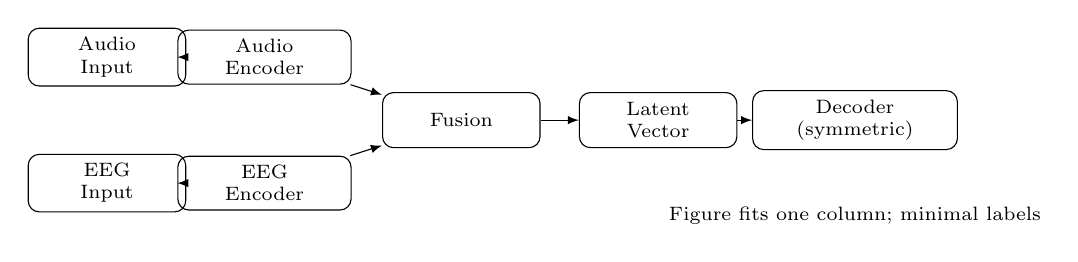
\begin{tikzpicture}[font=\scriptsize, >=latex, every node/.style={align=center}]
  % coordinates chosen to fit ~\columnwidth and keep height small
  \node[draw, rounded corners, minimum height=6mm, minimum width=20mm] (Ainput) at (-4.5,0.8) {Audio\\Input};
  \node[draw, rounded corners, minimum height=6mm, minimum width=22mm] (Aenc) at (-2.5,0.8) {Audio\\Encoder};

  \node[draw, rounded corners, minimum height=6mm, minimum width=20mm] (Einput) at (-4.5,-0.8) {EEG\\Input};
  \node[draw, rounded corners, minimum height=6mm, minimum width=22mm] (EEG) at (-2.5,-0.8) {EEG\\Encoder};

  \node[draw, rounded corners, minimum height=7mm, minimum width=20mm] (FUS) at (0,0) {Fusion};
  \node[draw, rounded corners, minimum height=7mm, minimum width=20mm] (Z) at (2.5,0) {Latent\\Vector};
  \node[draw, rounded corners, minimum height=7mm, minimum width=26mm] (Dec) at (5,0) {Decoder\\(symmetric)};

  % arrows
  \draw[->] (Ainput) -- (Aenc);
  \draw[->] (Einput) -- (EEG);
  \draw[->] (Aenc) -- (FUS);
  \draw[->] (EEG) -- (FUS);
  \draw[->] (FUS) -- (Z);
  \draw[->] (Z) -- (Dec);

  % note
  \node[below=6mm of Dec, font=\scriptsize, anchor=north] (note) {Figure fits one column; minimal labels};
\end{tikzpicture}

  \caption{SNN autoencoder architecture.  Input window $x$ is encoded and
  pre-processed by mode $\phi$, then compressed to latent $z \in \mathbb{R}^{32}$
  by the encoder (Linear+Leaky layers).  The decoder (LeakyInt+Linear)
  reconstructs $\hat{x}$.}
  \label{fig:arch}
\end{figure}

% ── Training ──────────────────────────────────────────────────
\subsection{Training}

\par All trained models minimize MSE reconstruction loss via Adam
\cite{kingma2015adam} ($\eta = 10^{-3}$, $\beta_1=0.9$, $\beta_2=0.999$).
SNN biophysical parameters ($R$, $C$, $V_{th}$) use a scaled learning rate
$\eta_{\mathrm{bio}} = 0.1\,\eta$ to stabilize membrane-dynamics optimization
\cite{neftci2019surrogate}; $R$ and $C$ are clamped to $10^{-6}$ in the
forward pass with gradients zeroed in the clamped region.
BPTT \cite{werbos1990backpropagation} propagates gradients through the full
time dimension. Early stopping monitors a held-out monitor MSE with patience
$P=5$ epochs and minimum delta $10^{-8}$ over a maximum of 30 epochs
\cite{eshraghian2023training}. Batch size is 1 to accommodate stateful
sequence processing. Each configuration is trained with five random seeds
($42$--$46$).

\par \textbf{Per-fold hyperparameter selection (SNN).} Within each outer fold,
the full SNN grid --- pre-processing mode
$\in\{\text{dense, conv1d, recurrent}\}$, threshold
$V_{th}\in\{0.5,1.0,1.5\}$, membrane decay $\alpha\in\{0.8,0.9,0.99\}$, three
encodings --- is trained on that fold's four training speakers and scored on the
inner validation speaker. The configuration with the lowest validation MSE is
selected, then \emph{retrained} on the training and validation speakers combined
and evaluated \emph{once} on the held-out test speaker. Because train and
validation speakers share no recordings with the test speaker but not with each
other, the retrain's early-stopping monitor is a recording-disjoint slice carved
(seeded, whole recordings) from the training speakers, so no test-speaker signal
ever reaches a fitting or stopping decision. The per-fold selected configuration
and its inner-validation scores are written to a selection manifest and
summarized in Table~\ref{tab:snnsel}.

\par \textbf{Fixed-architecture baselines.} LSTM-AE, GRU-AE, and Transformer-AE
use fixed profile architectures; their only use of the validation speaker is
early stopping, which never touches the test speaker. PCA and the mean-frame
predictor are fitted per fold on the training speakers only.

% ── Computational cost ────────────────────────────────────────
\subsection{Analytic computational cost}
\label{sec:energy}

\par We report an analytic \emph{computational-cost} figure, not an energy
measurement. The primary quantity is the raw operation count
\begin{equation}
  C_{\mathrm{raw}} = \sum_k N_k,
  \label{eq:craw}
\end{equation}
where $N_k$ is the number of operations of class $k$ executed in one forward pass
over a window. We count, separately, the following classes: for the ANN models,
dense multiply--accumulates (MACs), nonlinearity evaluations, attention
$QK^{\top}$/$\cdot\,V$ products, and normalization operations; for the SNN,
synaptic accumulations, neuron-state updates, and spike/event operations. The
event-driven classes are scaled by the measured mean spike fraction
$r\in[0,1]$ of the evaluated run, so an SNN that never spikes contributes no
event-operation cost.

\par As a secondary, explicitly labelled \emph{sensitivity analysis} we also
report a weighted proxy
\begin{equation}
  C_{\mathrm{weighted}} = \sum_k w_k N_k,
  \label{eq:cweighted}
\end{equation}
under a stated choice of relative per-class weights $w_k$; the ranking of models
under $C_{\mathrm{weighted}}$ is reported only alongside the weights that produce
it, never as a standalone claim.

\par Neither $C_{\mathrm{raw}}$ nor $C_{\mathrm{weighted}}$ is energy. Real energy
on a given device is dominated by memory movement, cache and SIMD behaviour, clock
frequency, supply voltage, exploited sparsity, and the target silicon
(CPU, GPU, or neuromorphic). On-device power measurement is future work; the
figures here are design-time guidance for comparing architectures under matched
software and a single CPU backend.

% ─────────────────────────────────────────────────────────────
\section{Experimental Setup}
\label{sec:setup}

\textbf{Dataset.}
\par The Free Spoken Digit Dataset (FSDD) \cite{jackson2018fsdd} contains
recordings of spoken digits (0--9) from six speakers at 8\,kHz. Each recording
is partitioned into non-overlapping windows of $T=256$ samples ($32\,$ms) with
stride $S=T$, so consecutive windows share no samples; the full dataset is used
(no window-count cap). Adjacent windows of one recording remain temporally
correlated, which motivates the recording-level statistical unit
(Sec.~\ref{sec:stats}).

\textbf{Preprocessing.}
\par Each window is z-score normalised in place (subtract mean, divide by
standard deviation) before encoding --- a per-window statistic, so it introduces
no cross-window leakage. Encodings that require a $[0,1]$ range (Poisson,
latency) re-normalise the z-scored window to its own $(x_{\min}, x_{\max})$
range internally. The three encodings are deterministic transforms (Poisson uses
a per-window seeded draw) and are not fitted.

\textbf{Nested leave-one-speaker-out cross-validation.}
\par The six speakers are assigned deterministic indices $0$--$5$. For outer
fold $f \in \{0,\dots,5\}$ the test speaker is $f$, the validation speaker is
$(f+1)\bmod 6$, and the remaining four speakers are the training set. Every
window is assigned to a split \emph{by its speaker, before any pooling};
training windows are shuffled (seeded), validation and test windows kept in
$(\text{recording},\text{position})$ order. Each speaker is the test speaker
exactly once and the validation speaker exactly once. At run start the harness
asserts that no \texttt{recording\_id} and no speaker appears in more than one
split and writes a per-fold split manifest (speaker sets, per-recording window
counts, content hashes); a violation aborts the run. Headline numbers come only
from the test-speaker split, aggregated across the six folds.

\begin{figure}[!t]
\centering
% Signal windowing diagram: non-overlapping T=256 windows, stride S=T
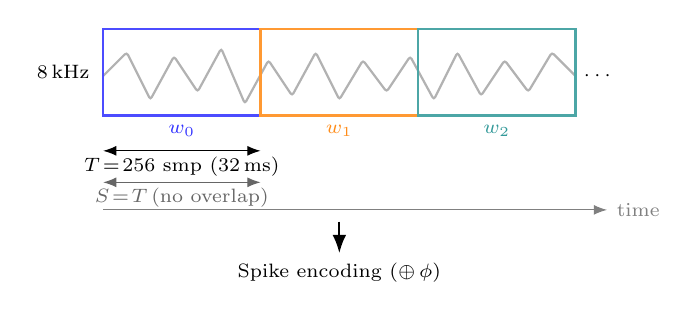
\begin{tikzpicture}[font=\scriptsize, >=Latex]

  % ── Raw waveform ──────────────────────────────────────────────────────
  \node[anchor=east] at (-0.05, 0.55) {8\,kHz};

  % Simplified zigzag waveform across 60mm
  \draw[gray!60, thick, rounded corners=1pt]
    (0.0,0.50) -- (0.3,0.80) -- (0.6,0.20) -- (0.9,0.75) -- (1.2,0.30) --
    (1.5,0.85) -- (1.8,0.15) -- (2.1,0.70) -- (2.4,0.25) -- (2.7,0.80) --
    (3.0,0.20) -- (3.3,0.70) -- (3.6,0.30) -- (3.9,0.75) -- (4.2,0.20) --
    (4.5,0.80) -- (4.8,0.25) -- (5.1,0.70) -- (5.4,0.30) -- (5.7,0.80) --
    (6.0,0.50);

  % Ellipsis continuation
  \node at (6.3, 0.50) {$\cdots$};

  % ── Window boxes ──────────────────────────────────────────────────────
  % W0: x in [0, 2.0]
  \draw[blue!70, thick] (0.0, 0.0) rectangle (2.0, 1.1);
  \node[blue!80, anchor=north] at (1.0, 0.0) {$w_0$};

  % W1: x in [2.0, 4.0]
  \draw[orange!80, thick] (2.0, 0.0) rectangle (4.0, 1.1);
  \node[orange!90, anchor=north] at (3.0, 0.0) {$w_1$};

  % W2: x in [4.0, 6.0]
  \draw[teal!70, thick] (4.0, 0.0) rectangle (6.0, 1.1);
  \node[teal!80, anchor=north] at (5.0, 0.0) {$w_2$};

  % ── Dimension braces ──────────────────────────────────────────────────
  % Window size T=256 (under W0)
  \draw[<->, black] (0.0, -0.45) -- (2.0, -0.45)
    node[midway, anchor=north, inner sep=2pt] {$T\!=\!256$ smp (32\,ms)};

  % Stride S=T (from start of W0 to start of W1)
  \draw[<->, black!60] (0.0, -0.85) -- (2.0, -0.85)
    node[midway, anchor=north, inner sep=2pt] {$S\!=\!T$\,(no overlap)};

  % ── Time axis arrow ───────────────────────────────────────────────────
  \draw[->, gray] (0.0, -1.20) -- (6.4, -1.20)
    node[anchor=west] {time};

  % ── Downward arrow to encoding ─────────────────────────────────────────
  \draw[->, thick] (3.0, -1.35) -- (3.0, -1.75);
  \node[anchor=north, align=center] at (3.0, -1.75)
    {Spike encoding $(\oplus\,\phi)$};

\end{tikzpicture}

\caption{Signal windowing. Each recording is segmented into non-overlapping
windows of $T=256$ samples (32\,ms at 8\,kHz). Stride $S=T$ yields
windows with no shared samples. Windows are assigned to train / validation /
test splits by speaker before any pooling.}
\label{fig:windowing}
\end{figure}

\textbf{Evaluation harness.}
\par The C++ harness \cite{furlan2026doi} runs on the XTensor backend
\cite{xtensor} (CPU-only, CBLAS, SIMD via xsimd). All models --- spiking and
non-spiking --- are trained and timed on this one backend, so the training and
inference times in Table~\ref{tab:perf} are directly comparable.

\textbf{Metrics.}
\par Per run we report reconstruction quality (MSE, MAE, $R^2$) and, for cost,
spike rate (SNN only; $0$ for the non-spiking models), the raw per-class
operation count of Sec.~\ref{sec:energy}, parameter count, training time, and
inference time in ms. FSDD provides no anomaly labels, so classification metrics
are out of scope. Reconstruction error in the headline tables is the mean $\pm$
sample standard deviation over the five seeds (per-seed means first); the
inferential analysis is in Sec.~\ref{sec:stats}. A per-window error record
(model, encoding, fold, split, speaker, recording, window, MSE, MAE) is written
for every model so that paired comparisons can be formed at the window,
recording, speaker, or seed level.

\textbf{Profile.}
\par A single JSON profile (\texttt{article-loso.json}) configures the harness:
full FSDD, six outer folds, five seeds, the four trained families plus the two
linear references, three encodings, and the SNN selection grid
($3\times3\times3$). The run script iterates the outer fold index; a profile
audit test verifies the profile parses and validates.

\begin{figure}[!t]
  \centering
  % Experiment execution pipeline flowchart (single-column)
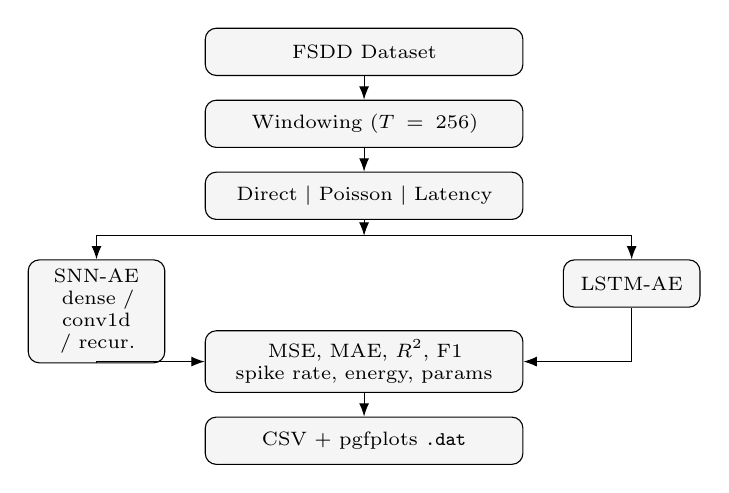
\begin{tikzpicture}[
  font=\scriptsize, >=Latex,
  node distance = 3mm and 2mm,
  box/.style  = {draw, rounded corners, align=center,
                 minimum height=6mm, fill=gray!8},
  main/.style = {box, text width=38mm, minimum width=40mm},
  side/.style = {box, text width=15mm, minimum width=17mm}
]

\node[main] (fsdd) {FSDD Dataset};
\node[main, below=of fsdd] (win)  {Windowing ($T=256$)};
\node[main, below=of win]  (enc)  {Direct \textbar{} Poisson \textbar{} Latency};

\node[side, below left  = 5mm and 5mm of enc] (snn)
  {SNN-AE\\dense / conv1d / recur.};
\node[side, below right = 5mm and 5mm of enc] (lstm) {LSTM-AE};

\node[main, below = 14mm of enc] (met)
  {MSE, MAE, $R^2$, F1\\spike rate, energy, params};
\node[main, below=of met] (out) {CSV + pgfplots \texttt{.dat}};

\draw[->] (fsdd) -- (win);
\draw[->] (win)  -- (enc);
\draw[->] (enc.south) -- ++(0,-2mm) coordinate (fork);
\draw[->] (fork) -| (snn.north);
\draw[->] (fork) -| (lstm.north);
\draw[->] (snn.south)  |- (met.west);
\draw[->] (lstm.south) |- (met.east);
\draw[->] (met) -- (out);

\end{tikzpicture}

  \caption{Experiment execution pipeline. Per outer fold, each FSDD window is
  encoded three ways and processed by the four trained families (SNN-AE with a
  per-fold selection sweep; LSTM-AE, GRU-AE, Transformer-AE fixed) plus the PCA
  and mean-frame references. Per-window errors and manifests are written to CSV
  and JSON.}
  \label{fig:flow}
\end{figure}

% ── Statistical methods ───────────────────────────────────────
\subsection{Statistical methods}
\label{sec:stats}

\par Comparisons are paired on a shared, model-independent window identifier, so
every model reconstructs the same windows and differences are formed per window.
Let $\mathrm{MSE}_{m,i}$ be the error of model $m$ on window $i$.

\par \textbf{Primary --- recording level.} For a recording $r$, let
$E_{m,r} = \operatorname{mean}_{i \in r}\mathrm{MSE}_{m,i}$. For model $m$ and
reference $b$ the paired difference is $d_r = E_{m,r} - E_{b,r}$. We report
$\operatorname{mean}(d_r)$, a $95\%$ confidence interval from a bootstrap that
resamples recordings, the Wilcoxon signed-rank $p$-value on $\{d_r\}$, and
Holm--Bonferroni correction across the reference set
$b \in \{\text{LSTM-AE, GRU-AE, Transformer-AE, PCA, Mean}\}$. Effect size is
reported both absolute ($\operatorname{mean}(d_r)$) and relative
($\operatorname{mean}(d_r)/\operatorname{mean}(E_{b,\cdot})$). Recordings are the
smallest unit across which windows are not, by construction, near-duplicates.

\par \textbf{Robustness --- speaker level.} Per held-out speaker (one per fold,
$n=6$) we form the mean error and run a paired Wilcoxon / sign test. This checks
whether the sign and rough magnitude of a difference hold across the six FSDD
speakers; with $n=6$ it is not strong population-level inference and is reported
as such.

\par \textbf{Descriptive --- window level.} Paired bootstrap on all windows,
reported but explicitly labelled pseudoreplicated (adjacent windows of a
recording are correlated), so it is never the basis of a claim.

\par \textbf{Robustness --- seed level.} Paired Wilcoxon across the five
per-seed mean errors, characterizing optimization/reproducibility variation
around the estimate.

\par The per-run CSVs are immutable; aggregation and statistics are separate
downstream steps that never overwrite them. Synthetic known-answer tests
(identical predictions $\Rightarrow p\approx1$ and CI spanning $0$; injected
constant offset $\Rightarrow$ significant with CI excluding $0$ and recovered
offset; label permutation $\Rightarrow$ approximately uniform $p$) guard the
analysis code in continuous integration.

% ─────────────────────────────────────────────────────────────
\section{Results}
\label{sec:results}

\par All numbers in this section come from the held-out test speaker only,
pooled across the six outer folds, and are reported as mean $\pm$ sample
standard deviation over the five seeds. Reconstruction quality is in
Table~\ref{tab:perf} (per model) and Table~\ref{tab:recon} (per model $\times$
encoding); Fig.~\ref{fig:results} plots the per-encoding test MSE with seed
error bars. Table~\ref{tab:snnsel} records which SNN pre-processing mode won on
each fold's validation speaker, and Table~\ref{tab:sig} gives the
recording-level paired analysis.

\subsection{Reconstruction quality}

% Source: data/paper_loso_summary.csv + data/paper_loso_recon_by_encoding.csv,
% from scripts/pipeline/guayaquil/02_guayaquil_build_loso_paper_data.py.
% Numeric claims below are regenerated from the run; see the table cells.
\par Table~\ref{tab:perf} reports test-speaker MSE, MAE, and $R^2$ for the four
trained families and the two linear references, with each model's real
parameter count and raw operation count $C_{\mathrm{raw}}$
(Sec.~\ref{sec:energy}). The mean-frame predictor and PCA fix the scale of a
"no-model" and a "best linear" reference; a trained model is only interesting to
the extent it beats PCA. Table~\ref{tab:recon} breaks the same quantities down
by input encoding.

\par \emph{Interpretation is deferred to the regenerated tables:} the earlier,
leakage-affected version of this study over-stated the SNN advantage because
train and validation windows shared speakers and recordings with the test
windows. Under speaker-disjoint nested evaluation the reference points (PCA,
mean-frame) and the recording-level intervals in Table~\ref{tab:sig} determine
which differences survive.

\subsection{Per-fold model selection}
\par Table~\ref{tab:snnsel} lists, for each outer fold and encoding, the SNN
pre-processing mode, threshold, and decay selected on that fold's validation
speaker. Because selection is redone inside every fold, the SNN result is the
performance of a \emph{selection procedure}, not of a single hand-picked
configuration; disagreement of the selected mode across folds is itself a
finding about how encoding-dependent the best pre-processing is.

\subsection{Computational cost and timing}
% Source: data/paper_loso_summary.csv (params, craw, train_ms, infer_ms columns).
\par Table~\ref{tab:perf} also carries wall-clock training and inference time,
measured for every model on the one XTensor/CPU backend, and the raw operation
count. The recurrent baselines and the SNN cost $O(T d H)$ per window; the
Transformer additionally pays the $O(T^2 d_{\mathrm{model}})$ self-attention
interaction term, which is reflected in its $C_{\mathrm{raw}}$ column
independently of its MSE. The weighted proxy $C_{\mathrm{weighted}}$
(Eq.~\eqref{eq:cweighted}) is reported in the released JSON as a labelled
sensitivity analysis and is not used for any claim here.

% Source: data/paper_loso_summary.csv, from
% scripts/pipeline/guayaquil/02_guayaquil_build_loso_paper_data.py (test-split rows,
% mean +/- sample std over the 5 seeds; best cell per column in \textbf{}).
\begin{table*}[!t]
\caption{Test-speaker reconstruction and cost by model, pooled over the six
outer folds (mean $\pm$ std over five seeds; best per column in bold). $P$ is the
real trainable-parameter count; $C_{\mathrm{raw}}$ is the raw per-forward-pass
operation count of Sec.~\ref{sec:energy}. PCA and Mean are analytic references
(no training, no parameter count).}
\centering\small
\pgfplotstabletypeset[
  col sep=semicolon,
  columns={model,mse,mae,r2,params,craw,train_ms,infer_ms},
  columns/model/.style={string type,column name=Model},
  columns/mse/.style={string type,column type={r},column name=MSE},
  columns/mae/.style={string type,column type={r},column name=MAE},
  columns/r2/.style={string type,column type={r},column name=$R^2$},
  columns/params/.style={string type,column type={r},column name=$P$},
  columns/craw/.style={string type,column type={r},column name=$C_{\mathrm{raw}}$},
  columns/train_ms/.style={string type,column type={r},column name=Train\,(ms)},
  columns/infer_ms/.style={string type,column type={r},column name=Infer\,(ms)},
  every head row/.style={before row=\toprule,after row=\midrule},
  every last row/.style={after row=\bottomrule}
]{data/paper_loso_summary.csv}%
\label{tab:perf}
\end{table*}

% Source: data/paper_loso_recon_by_encoding.csv (same provenance as tab:perf).
\begin{table}[!t]
\caption{Test-speaker reconstruction per input encoding
(mean $\pm$ std over five seeds).}
\centering\small
\pgfplotstabletypeset[
  col sep=semicolon,
  columns={model,encoding,mse,mae,r2},
  columns/model/.style={string type,column name=Model},
  columns/encoding/.style={string type,column name=Encoding},
  columns/mse/.style={string type,column type={r},column name=MSE},
  columns/mae/.style={string type,column type={r},column name=MAE},
  columns/r2/.style={string type,column type={r},column name=$R^2$},
  every head row/.style={before row=\toprule,after row=\midrule},
  every last row/.style={after row=\bottomrule}
]{data/paper_loso_recon_by_encoding.csv}
\label{tab:recon}
\end{table}

% Source: data/paper_loso_snn_selection.tex, from
% scripts/pipeline/guayaquil/02_guayaquil_build_loso_paper_data.py (modal winning
% mode per fold x encoding; median V_th / alpha over seeds).
\begin{table}[!t]
\caption{SNN pre-processing mode, threshold, and decay selected on each outer
fold's validation speaker. A parenthesised fraction marks folds where the seeds
did not unanimously select the same mode.}
\centering\small
% placeholder — regenerated by 02_guayaquil_build_loso_paper_data.py
\begin{tabular}{llllrrr}
\toprule
Fold & Test spk. & Val spk. & Enc. & Mode & $V_{th}$ & $\alpha$ \\
\midrule
0 & --- & --- & --- & --- & --- & --- \\
\bottomrule
\end{tabular}

\label{tab:snnsel}
\end{table}

% Source: data/article_loso_significance_recording.tex, from
% scripts/pipeline/guayaquil/04_guayaquil_significance_tests.py (recording-level
% paired difference d_r; bootstrap over recordings; Holm across references).
\begin{table}[!t]
\caption{Recording-level paired analysis on the test speakers. $\overline{d_r}$
is the mean per-recording MSE difference (model $-$ reference); a negative value
favours the model. CI is a $95\%$ bootstrap interval over recordings;
$p_{\text{Holm}}$ is the Holm-corrected Wilcoxon signed-rank $p$-value.}
\centering\small
\input{data/article_loso_significance_recording.tex}
\label{tab:sig}
\end{table}

% Source: data/paper_loso_mse_plot.csv (wide: encoding, then one MSE column per
% model), read by figs/fig_results.tex.
\begin{figure}[!t]
  \centering
  % Test-speaker MSE by model and encoding, from the nested-LOSO run.
% data/paper_loso_mse_plot.csv is wide: encoding, then one MSE column per model
% (mean, pca, snn_ae, lstm_ae, gru_ae, transformer_ae). The mean-frame column is
% omitted here for vertical scale.
\pgfplotstableread[col sep=comma]{data/paper_loso_mse_plot.csv}\msetable

\begin{tikzpicture}[font=\scriptsize]
  \begin{axis}[
    ybar=1.5pt,
    bar width=4pt,
    width=\columnwidth,
    height=4.2cm,
    ymin=0,
    enlarge x limits=0.25,
    legend style={at={(0.5,-0.32)}, anchor=north, legend columns=3,
      /tikz/every even column/.append style={column sep=3pt}},
    symbolic x coords={direct,poisson,latency},
    xtick=data,
    ylabel={test MSE},
    ymajorgrids]
    \addplot+[fill=black!25] table[x=encoding,y=pca] {\msetable};
    \addplot+[fill=green!60] table[x=encoding,y=snn_ae] {\msetable};
    \addplot+[fill=black!70] table[x=encoding,y=lstm_ae] {\msetable};
    \addplot+[fill=blue!55]  table[x=encoding,y=gru_ae] {\msetable};
    \addplot+[fill=red!50]   table[x=encoding,y=transformer_ae] {\msetable};
    \legend{PCA, SNN-AE, LSTM-AE, GRU-AE, Transformer-AE}
  \end{axis}
\end{tikzpicture}

  \caption{Test-speaker MSE by model and input encoding (mean over seeds and
  folds; the mean-frame reference is omitted for scale). Error bars, where
  shown, are $\pm1$ seed standard deviation.}
  \label{fig:results}
\end{figure}

% ─────────────────────────────────────────────────────────────
\section{Discussion}
\label{sec:discussion}

\par Two things should be read from Table~\ref{tab:sig} rather than from raw MSE
gaps. First, whether each trained family beats the PCA reference at all: under
speaker-disjoint evaluation, a family whose recording-level interval against PCA
includes zero has not demonstrated that its nonlinearity buys anything on this
benchmark. Second, the ordering among SNN-AE, LSTM-AE, GRU-AE, and Transformer-AE
--- a difference is only asserted where the Holm-corrected interval excludes
zero. The seed-level and speaker-level ($n=6$) checks in the released JSON say
whether an ordering that holds in the pooled recording-level analysis also holds
run-to-run and speaker-to-speaker.

\par The encoding comparison (Table~\ref{tab:recon}) is where an SNN-specific
effect is most likely to appear, because the encoding only reshapes the SNN's
input; the non-spiking baselines consume the same framed window regardless. If
latency or Poisson coding helps the SNN relative to direct coding, that is a
property of spike-based representation, not of the reconstruction task.

\par The cost picture is separable from the quality picture. The
operation-count column of Table~\ref{tab:perf} orders the models by arithmetic
work under matched software; the self-attention $O(T^2 d_{\mathrm{model}})$ term
makes the Transformer's per-window cost grow faster in sequence length than the
recurrent models', independent of which model reconstructs best. Wall-clock
timing on the shared CPU backend is reported alongside, but it reflects this
implementation and backend, not silicon-level energy.

\emph{Limitations.}
\begin{itemize}
  \item \textbf{Six speakers.} FSDD has six speakers, so the speaker-level
        analysis has $n=6$ and is a robustness check, not population inference;
        the recording-level analysis is the primary estimand for this reason.
  \item \textbf{Single dataset.} Only FSDD is used; the ranking may not transfer
        to other 1-D signal domains.
  \item \textbf{Cost is not energy.} $C_{\mathrm{raw}}$ and $C_{\mathrm{weighted}}$
        count operations under matched software; real energy depends on memory
        movement, sparsity exploitation, and target hardware. On-device
        measurement is future work.
  \item \textbf{Correlated windows.} Non-overlapping windows of one recording
        remain correlated, so window-level statistics are pseudoreplicated and
        used descriptively only.
  \item \textbf{Approximate parameter matching.} The Transformer-AE is sized
        \emph{near}, not equal to, the recurrent baselines; Table~\ref{tab:perf}
        reports the real counts so cost and quality can be read together.
\end{itemize}

\par All results are loaded directly from experiment-generated CSV files; the
per-run CSVs are immutable and aggregation never overwrites them.

\IEEEtriggeratref{13}
% ─────────────────────────────────────────────────────────────
\section{Conclusion}
\label{sec:conclusion}

\par We compared four trained autoencoder families --- SNN-AE, LSTM-AE, GRU-AE,
and a bottlenecked Transformer-AE --- under three spike-encoding front ends,
against PCA and mean-frame linear references, for 1-D temporal signal
reconstruction on FSDD. The evaluation is leakage-controlled: nested six-fold
leave-one-speaker-out cross-validation with no recording or speaker crossing a
split and SNN hyperparameters selected on the inner validation speaker only.
Differences are reported at the recording level with bootstrap intervals and
Holm-corrected tests, with speaker- and seed-level results as robustness
evidence; cost is an analytic per-class operation count, explicitly not an
energy measurement. This design directly answers the leakage, missing-baseline,
missing-significance, and energy-overclaim objections to the earlier version of
this study. The harness, profiles, and analysis scripts are released so the
protocol can be reused for other 1-D signal families.

\bibliographystyle{IEEEtran}
\bibliography{paper}

\end{document}
